\documentclass{article}
\usepackage[utf8]{inputenc}
\usepackage{url}

\title{Assignment 1 EECS 410}
\author{Madison Hillyard }
\date{September 15, 2020}

\usepackage{natbib}
\usepackage{graphicx}
\usepackage{float}

\begin{document}

\maketitle

\section{Introduction}
This assignment covered the creation of an Android Application. The main function of this application is to sample the device's real time internal accelerometer data, graph that data and retrieve the data in a csv file format. This includes both the associated $x$, $y$, and $z$ axis accelerometer data. The main tool used in graphing is the MPAndroidChart Library. \citep{MPACDocs} This extensible library allows for touch and gesture interaction with the Chart. 

To facilitate the exporting of the data out of the app, a file containing the accelerometer data is created and saved locally on the mobile device. Using the Intent Class the application then allows for the csv file to be shared using the user's personal google drive account. 

This application allows the user to visualize their device's internal acceleromenter data to better understand the device's sensed movement through space. This can be used to better the user's understanding of accelerometer sensors and the connection between their physical movement and acceleration on a three dimensional plane.

\section{Related Work}
In looking for another application that displays and samples internal device data, Physics Toolbox Accelerometer was the most closely related to this assignment's mission. This application has multiple options for visualizing the internal accelerometer data as well as multiple other sensors. The application also shows derived data like a vector view to interact with the data. This view furthers the goal of showing more uses and representation of the data gained from internal sensors.\citep{PhyToolBox}

\begin{figure}[H]
\centering
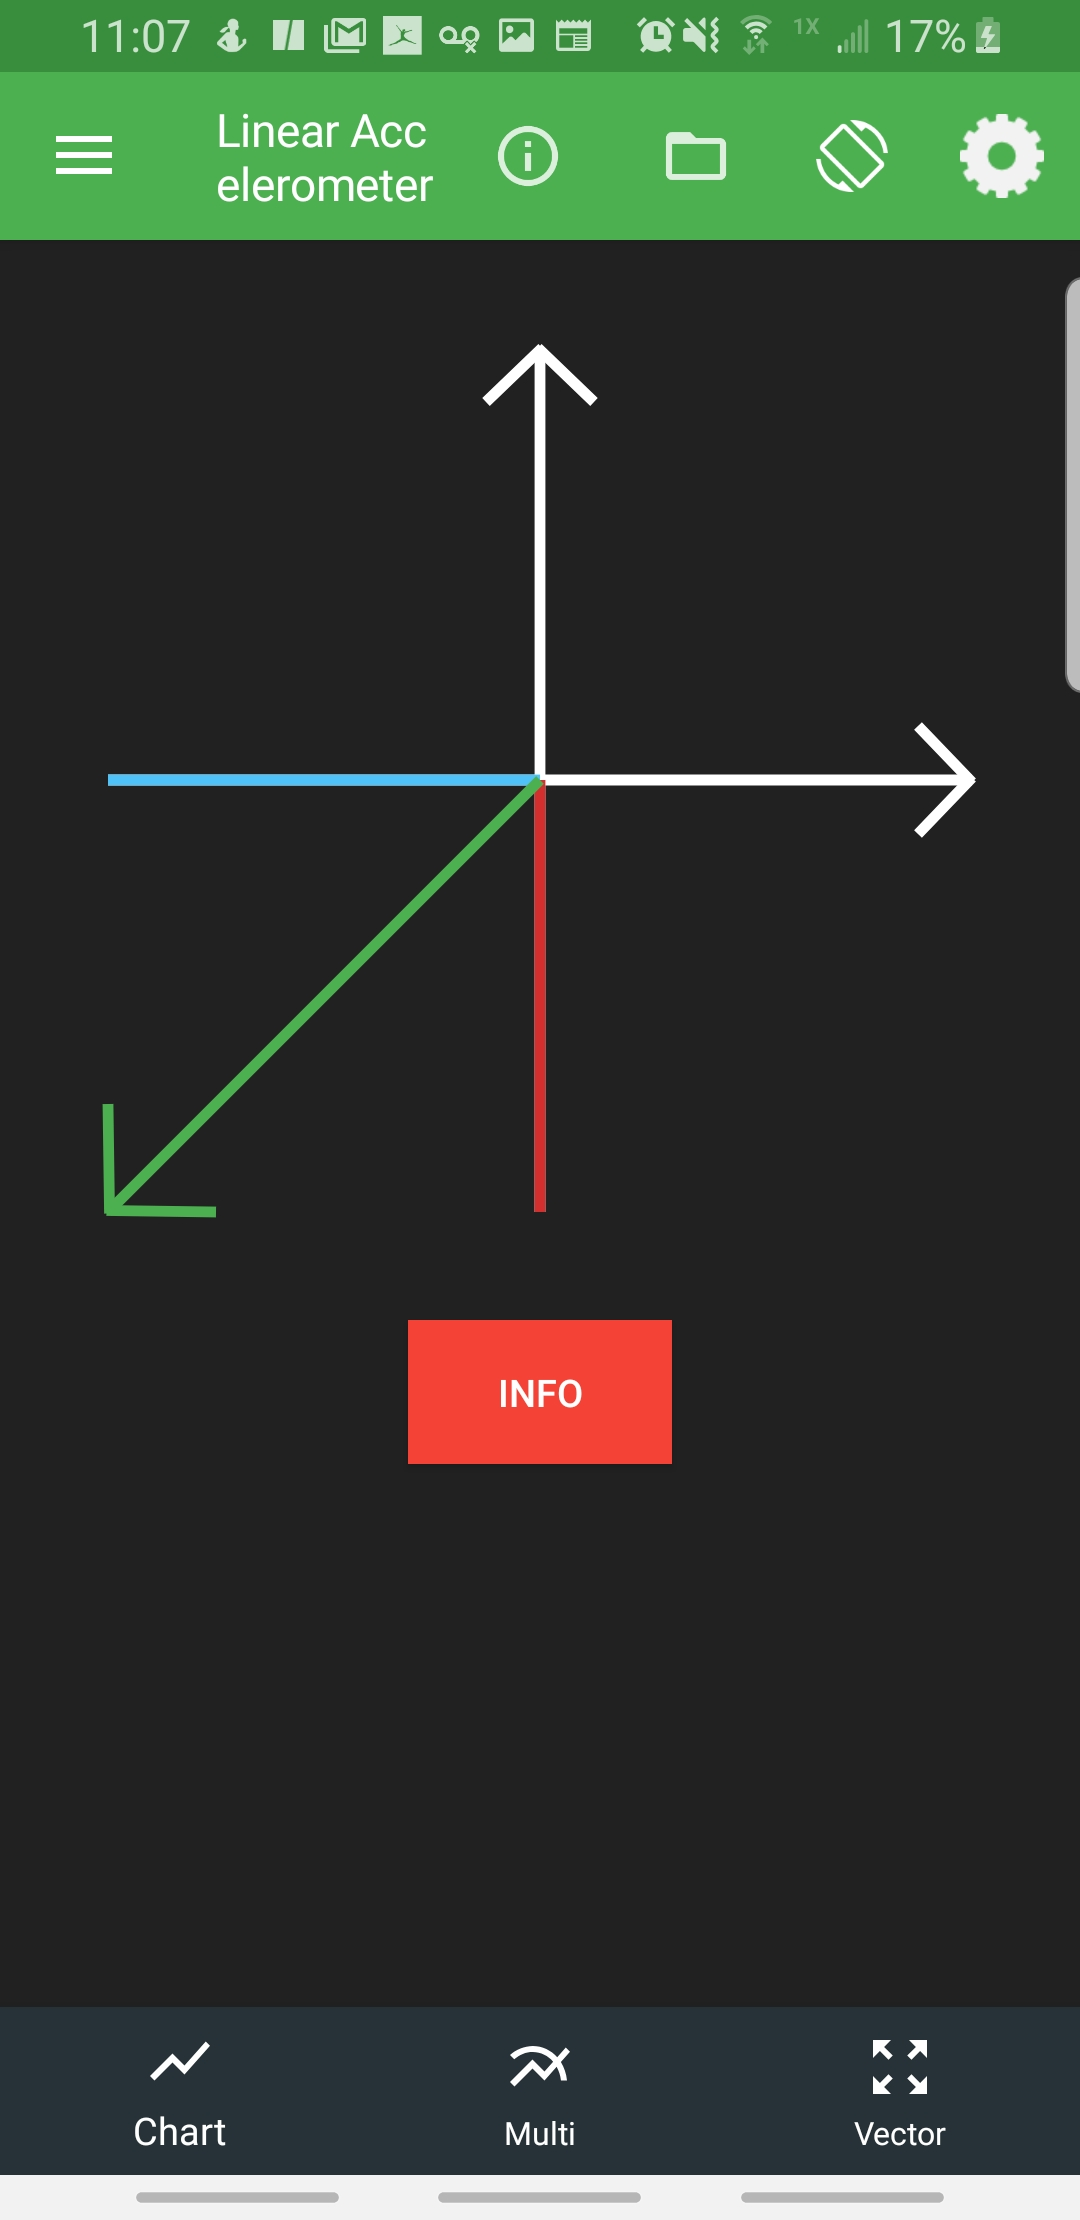
\includegraphics[scale= .07]{physicsToolBoxVector}
\caption{The vector view of internal accelerometer data form Physics Toolbox Accelerometer}
\label{fig:phyToolboxVecotor} 
\end{figure}

\section{System Overview}
The System has two states and three user inputs. The user inputs do not include the closing and pausing of app. The Pausing of the Application is the same as pausing the data sampling. The closing of the application is the same as resetting the data. 
\begin{figure}[H]
\centering
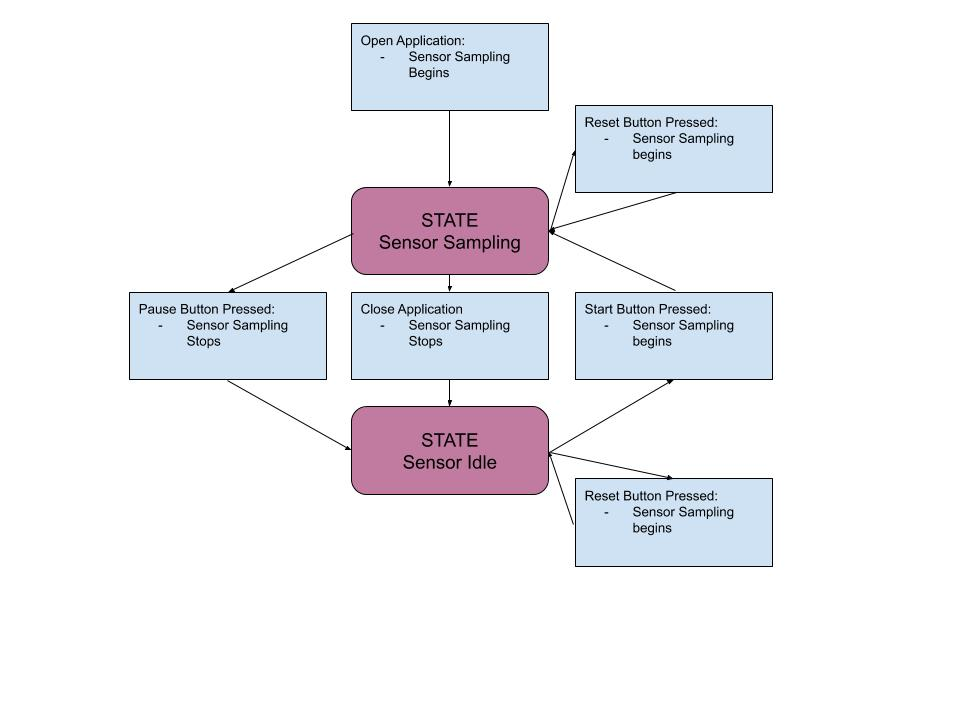
\includegraphics[scale=.30]{system.jpg}
\caption{The System}
\label{fig:system}
\end{figure}

\section{User Guide}
This Application has four main parts: Chart, Chart Controls, Current Data, and Export Button. 

\begin{figure}[H]
\centering
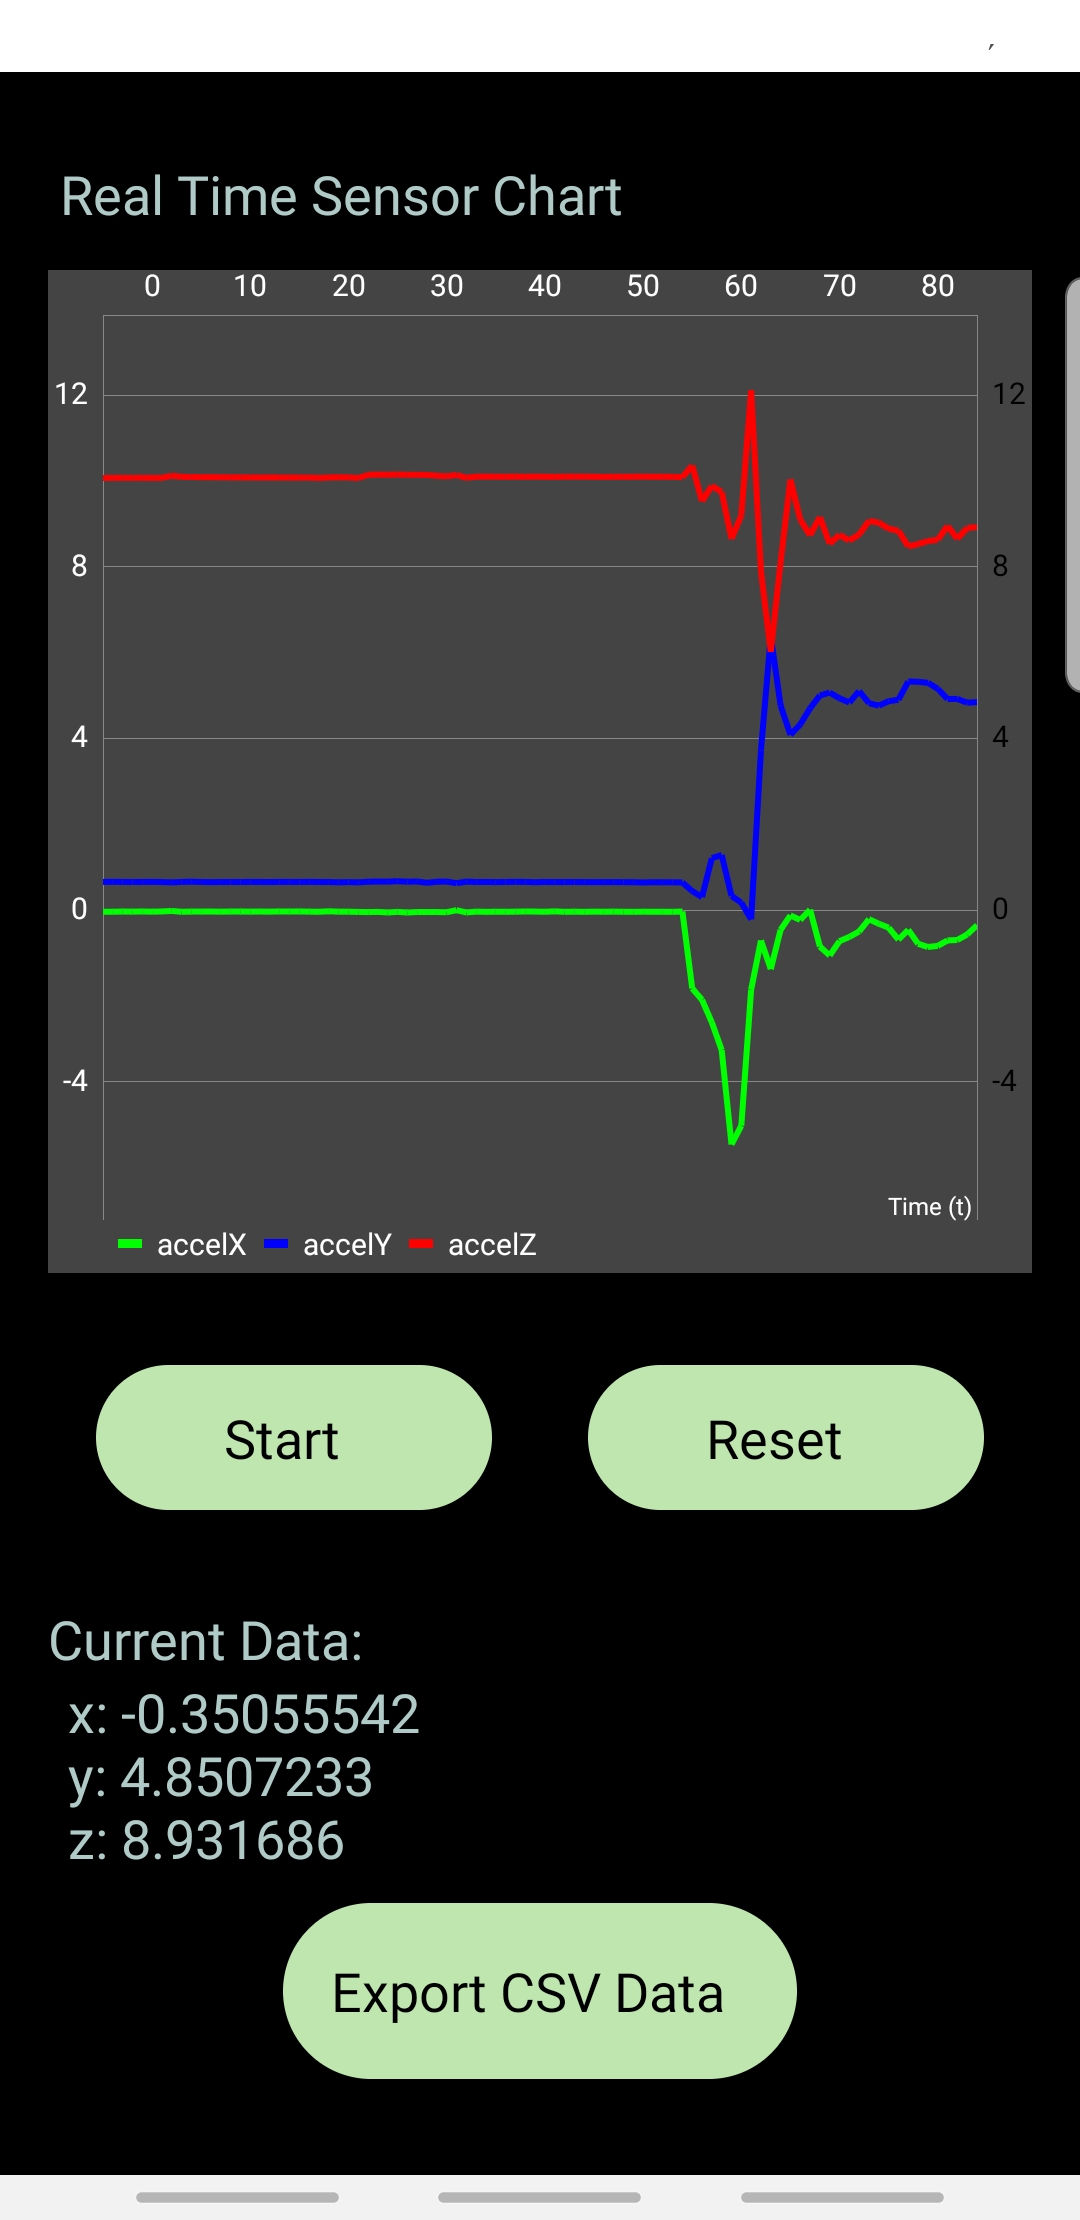
\includegraphics[scale= .1]{application.jpg}
\caption{The Application User Interface}
\label{fig:application} 
\end{figure}
\subsection{Chart}
The Chart itself is a simple line graph. The X-axis shows the data unit number while the Y-axis shows the internal  accelerometer data in $m/(s^2)$. The data is graphed using three different colored lines that are noted in the legend below the chart. Each line represents one axis of data either $x$, $y$, or $z$. The chart can be dragged and moved to better visualize the data. Each axis will resize using a pinching gesture. The chart will by default dynamically resize to show all the accelerometer data that has been sampled.
\subsection{Chart Controls}
The Chart Controls consist of two buttons. 
\subsubsection{Start/Pause}
This button toggles the application's data sampling state. It is labelled as either "Start" or "Pause" depending on the state of data sampling. To pause or start data sampling press this button.
\subsubsection{Reset}
This button resets the data shown on the chart. This also resets associated background data.
\subsection{Current Data}
The Current Data section shows the user the most recent data that is presented on the graph. The data that is shown is displayed separated into the $x$, $y$, and $z$ axis to coincide with the data representation on the chart.
\subsection{Export Button}
This button allows the user to export the data that has been sampled since the last reset. Sharing to Google Drive is encouraged but sharing by email and other sharing options enabled on the device is enabled using the application as well.

\section{Discussion}
This application could be a good tool for teaching students about physics and by extension the importance of physics in technology. This application could easily be extended to show the internal sensors used, for example in an app counting a user's steps, to calculate actionable information. The application Physics Toolbox Accelerometer discussed in the Related Work section is a good candidate for extending for this function too. The use and manipulation of multi-sensor system data to determine actionable application information could show very succinctly.

In designing this application there could be improved code modularity and scalability. In future iteration I hope to implement more robust code re-usability and User Interface Layout. The Layout that is currently in use is works on well on the screen dimensions of a Samsung Galaxy S8, but has not been tested on other layouts and screen sizes. In the future the utilization of a RelativeLayout rather than a LinearLayout will help to ensure cross compatibility. 

In the development of this application the Android Developer Studio Documentation website and multiple other sources were invaluable. The Sensor and SensorManager documentation contributed greatly to this effort. \citep{IntentDocs} When working on the export functionality the Tutorial Exporting CSV in Android - Android Studio Programming Tutorial was very helpful. \citep{exportTut} The Vogella Website was also very helpful by clearly explaining the foundations of Sensor Management on Android Devices. \citep{Vogella}

\section{Conclusion}
In further iterations of this application, a vector view like Figure 1 would be a good improvement. The use case of this application allows for many future improvements to make the connection between sensor data and actionable information. This has been a significant stride into Android Development and will be very interesting to build off of in the coming assignments. 

\bibliographystyle{plain}
\bibliography{references}
\end{document}
